% Options for packages loaded elsewhere
\PassOptionsToPackage{unicode}{hyperref}
\PassOptionsToPackage{hyphens}{url}
%
\documentclass[
]{article}
\usepackage{amsmath,amssymb}
\usepackage{lmodern}
\usepackage{iftex}
\ifPDFTeX
  \usepackage[T1]{fontenc}
  \usepackage[utf8]{inputenc}
  \usepackage{textcomp} % provide euro and other symbols
\else % if luatex or xetex
  \usepackage{unicode-math}
  \defaultfontfeatures{Scale=MatchLowercase}
  \defaultfontfeatures[\rmfamily]{Ligatures=TeX,Scale=1}
\fi
% Use upquote if available, for straight quotes in verbatim environments
\IfFileExists{upquote.sty}{\usepackage{upquote}}{}
\IfFileExists{microtype.sty}{% use microtype if available
  \usepackage[]{microtype}
  \UseMicrotypeSet[protrusion]{basicmath} % disable protrusion for tt fonts
}{}
\makeatletter
\@ifundefined{KOMAClassName}{% if non-KOMA class
  \IfFileExists{parskip.sty}{%
    \usepackage{parskip}
  }{% else
    \setlength{\parindent}{0pt}
    \setlength{\parskip}{6pt plus 2pt minus 1pt}}
}{% if KOMA class
  \KOMAoptions{parskip=half}}
\makeatother
\usepackage{xcolor}
\usepackage[margin=2.54cm]{geometry}
\usepackage{color}
\usepackage{fancyvrb}
\newcommand{\VerbBar}{|}
\newcommand{\VERB}{\Verb[commandchars=\\\{\}]}
\DefineVerbatimEnvironment{Highlighting}{Verbatim}{commandchars=\\\{\}}
% Add ',fontsize=\small' for more characters per line
\usepackage{framed}
\definecolor{shadecolor}{RGB}{248,248,248}
\newenvironment{Shaded}{\begin{snugshade}}{\end{snugshade}}
\newcommand{\AlertTok}[1]{\textcolor[rgb]{0.94,0.16,0.16}{#1}}
\newcommand{\AnnotationTok}[1]{\textcolor[rgb]{0.56,0.35,0.01}{\textbf{\textit{#1}}}}
\newcommand{\AttributeTok}[1]{\textcolor[rgb]{0.77,0.63,0.00}{#1}}
\newcommand{\BaseNTok}[1]{\textcolor[rgb]{0.00,0.00,0.81}{#1}}
\newcommand{\BuiltInTok}[1]{#1}
\newcommand{\CharTok}[1]{\textcolor[rgb]{0.31,0.60,0.02}{#1}}
\newcommand{\CommentTok}[1]{\textcolor[rgb]{0.56,0.35,0.01}{\textit{#1}}}
\newcommand{\CommentVarTok}[1]{\textcolor[rgb]{0.56,0.35,0.01}{\textbf{\textit{#1}}}}
\newcommand{\ConstantTok}[1]{\textcolor[rgb]{0.00,0.00,0.00}{#1}}
\newcommand{\ControlFlowTok}[1]{\textcolor[rgb]{0.13,0.29,0.53}{\textbf{#1}}}
\newcommand{\DataTypeTok}[1]{\textcolor[rgb]{0.13,0.29,0.53}{#1}}
\newcommand{\DecValTok}[1]{\textcolor[rgb]{0.00,0.00,0.81}{#1}}
\newcommand{\DocumentationTok}[1]{\textcolor[rgb]{0.56,0.35,0.01}{\textbf{\textit{#1}}}}
\newcommand{\ErrorTok}[1]{\textcolor[rgb]{0.64,0.00,0.00}{\textbf{#1}}}
\newcommand{\ExtensionTok}[1]{#1}
\newcommand{\FloatTok}[1]{\textcolor[rgb]{0.00,0.00,0.81}{#1}}
\newcommand{\FunctionTok}[1]{\textcolor[rgb]{0.00,0.00,0.00}{#1}}
\newcommand{\ImportTok}[1]{#1}
\newcommand{\InformationTok}[1]{\textcolor[rgb]{0.56,0.35,0.01}{\textbf{\textit{#1}}}}
\newcommand{\KeywordTok}[1]{\textcolor[rgb]{0.13,0.29,0.53}{\textbf{#1}}}
\newcommand{\NormalTok}[1]{#1}
\newcommand{\OperatorTok}[1]{\textcolor[rgb]{0.81,0.36,0.00}{\textbf{#1}}}
\newcommand{\OtherTok}[1]{\textcolor[rgb]{0.56,0.35,0.01}{#1}}
\newcommand{\PreprocessorTok}[1]{\textcolor[rgb]{0.56,0.35,0.01}{\textit{#1}}}
\newcommand{\RegionMarkerTok}[1]{#1}
\newcommand{\SpecialCharTok}[1]{\textcolor[rgb]{0.00,0.00,0.00}{#1}}
\newcommand{\SpecialStringTok}[1]{\textcolor[rgb]{0.31,0.60,0.02}{#1}}
\newcommand{\StringTok}[1]{\textcolor[rgb]{0.31,0.60,0.02}{#1}}
\newcommand{\VariableTok}[1]{\textcolor[rgb]{0.00,0.00,0.00}{#1}}
\newcommand{\VerbatimStringTok}[1]{\textcolor[rgb]{0.31,0.60,0.02}{#1}}
\newcommand{\WarningTok}[1]{\textcolor[rgb]{0.56,0.35,0.01}{\textbf{\textit{#1}}}}
\usepackage{graphicx}
\makeatletter
\def\maxwidth{\ifdim\Gin@nat@width>\linewidth\linewidth\else\Gin@nat@width\fi}
\def\maxheight{\ifdim\Gin@nat@height>\textheight\textheight\else\Gin@nat@height\fi}
\makeatother
% Scale images if necessary, so that they will not overflow the page
% margins by default, and it is still possible to overwrite the defaults
% using explicit options in \includegraphics[width, height, ...]{}
\setkeys{Gin}{width=\maxwidth,height=\maxheight,keepaspectratio}
% Set default figure placement to htbp
\makeatletter
\def\fps@figure{htbp}
\makeatother
\setlength{\emergencystretch}{3em} % prevent overfull lines
\providecommand{\tightlist}{%
  \setlength{\itemsep}{0pt}\setlength{\parskip}{0pt}}
\setcounter{secnumdepth}{-\maxdimen} % remove section numbering
\ifLuaTeX
  \usepackage{selnolig}  % disable illegal ligatures
\fi
\IfFileExists{bookmark.sty}{\usepackage{bookmark}}{\usepackage{hyperref}}
\IfFileExists{xurl.sty}{\usepackage{xurl}}{} % add URL line breaks if available
\urlstyle{same} % disable monospaced font for URLs
\hypersetup{
  pdftitle={ENV 790.30 - Time Series Analysis for Energy Data \textbar{} Spring 2023},
  pdfauthor={Yuxiang Ren},
  hidelinks,
  pdfcreator={LaTeX via pandoc}}

\title{ENV 790.30 - Time Series Analysis for Energy Data \textbar{}
Spring 2023}
\usepackage{etoolbox}
\makeatletter
\providecommand{\subtitle}[1]{% add subtitle to \maketitle
  \apptocmd{\@title}{\par {\large #1 \par}}{}{}
}
\makeatother
\subtitle{Assignment 3 - Due date 02/10/23}
\author{Yuxiang Ren}
\date{}

\begin{document}
\maketitle

\hypertarget{directions}{%
\subsection{Directions}\label{directions}}

You should open the .rmd file corresponding to this assignment on
RStudio. The file is available on our class repository on Github.

Once you have the file open on your local machine the first thing you
will do is rename the file such that it includes your first and last
name (e.g., ``LuanaLima\_TSA\_A02\_Sp23.Rmd''). Then change ``Student
Name'' on line 4 with your name.

Then you will start working through the assignment by \textbf{creating
code and output} that answer each question. Be sure to use this
assignment document. Your report should contain the answer to each
question and any plots/tables you obtained (when applicable).

Please keep this R code chunk options for the report. It is easier for
us to grade when we can see code and output together. And the tidy.opts
will make sure that line breaks on your code chunks are automatically
added for better visualization.

When you have completed the assignment, \textbf{Knit} the text and code
into a single PDF file. Submit this pdf using Sakai.

\hypertarget{questions}{%
\subsection{Questions}\label{questions}}

Consider the same data you used for A2 from the spreadsheet
``Table\_10.1\_Renewable\_Energy\_Production\_and\_Consumption\_by\_Source.xlsx''.
The data comes from the US Energy Information and Administration and
corresponds to the December 2022 \textbf{Monthly} Energy Review. Once
again you will work only with the following columns: Total Biomass
Energy Production, Total Renewable Energy Production, Hydroelectric
Power Consumption. Create a data frame structure with these three time
series only.

R packages needed for this assignment:``forecast'',``tseries'', and
``Kendall''. Install these packages, if you haven't done yet. Do not
forget to load them before running your script, since they are NOT
default packages.\textbackslash{}

\begin{Shaded}
\begin{Highlighting}[]
\CommentTok{\# Load/install required package}
\FunctionTok{library}\NormalTok{(forecast)}
\end{Highlighting}
\end{Shaded}

\begin{verbatim}
## Registered S3 method overwritten by 'quantmod':
##   method            from
##   as.zoo.data.frame zoo
\end{verbatim}

\begin{Shaded}
\begin{Highlighting}[]
\FunctionTok{library}\NormalTok{(tseries)}
\FunctionTok{library}\NormalTok{(Kendall)}
\FunctionTok{library}\NormalTok{(xlsx)}
\FunctionTok{library}\NormalTok{(formatR)}
\FunctionTok{library}\NormalTok{(ggplot2)}
\end{Highlighting}
\end{Shaded}

\begin{Shaded}
\begin{Highlighting}[]
\NormalTok{rawdata }\OtherTok{\textless{}{-}} \FunctionTok{read.xlsx}\NormalTok{(}\AttributeTok{file =} \StringTok{"./Data/Table\_10.1\_Renewable\_Energy\_Production\_and\_Consumption\_by\_Source.xlsx"}\NormalTok{,}
    \AttributeTok{header =} \ConstantTok{FALSE}\NormalTok{, }\AttributeTok{startRow =} \DecValTok{13}\NormalTok{, }\AttributeTok{sheetIndex =} \DecValTok{1}\NormalTok{)}
\NormalTok{read\_col\_names }\OtherTok{\textless{}{-}} \FunctionTok{read.xlsx}\NormalTok{(}\AttributeTok{file =} \StringTok{"./Data/Table\_10.1\_Renewable\_Energy\_Production\_and\_Consumption\_by\_Source.xlsx"}\NormalTok{,}
    \AttributeTok{header =} \ConstantTok{FALSE}\NormalTok{, }\AttributeTok{startRow =} \DecValTok{11}\NormalTok{, }\AttributeTok{endRow =} \DecValTok{11}\NormalTok{, }\AttributeTok{sheetIndex =} \DecValTok{1}\NormalTok{)}
\FunctionTok{colnames}\NormalTok{(rawdata) }\OtherTok{\textless{}{-}}\NormalTok{ read\_col\_names}
\FunctionTok{head}\NormalTok{(rawdata)}
\end{Highlighting}
\end{Shaded}

\begin{verbatim}
##        Month Wood Energy Production Biofuels Production
## 1 1973-01-01                129.630       Not Available
## 2 1973-02-01                117.194       Not Available
## 3 1973-03-01                129.763       Not Available
## 4 1973-04-01                125.462       Not Available
## 5 1973-05-01                129.624       Not Available
## 6 1973-06-01                125.435       Not Available
##   Total Biomass Energy Production Total Renewable Energy Production
## 1                         129.787                           403.981
## 2                         117.338                           360.900
## 3                         129.938                           400.161
## 4                         125.636                           380.470
## 5                         129.834                           392.141
## 6                         125.611                           377.232
##   Hydroelectric Power Consumption Geothermal Energy Consumption
## 1                         272.703                         1.491
## 2                         242.199                         1.363
## 3                         268.810                         1.412
## 4                         253.185                         1.649
## 5                         260.770                         1.537
## 6                         249.859                         1.763
##   Solar Energy Consumption Wind Energy Consumption Wood Energy Consumption
## 1            Not Available           Not Available                 129.630
## 2            Not Available           Not Available                 117.194
## 3            Not Available           Not Available                 129.763
## 4            Not Available           Not Available                 125.462
## 5            Not Available           Not Available                 129.624
## 6            Not Available           Not Available                 125.435
##   Waste Energy Consumption Biofuels Consumption
## 1                    0.157        Not Available
## 2                    0.144        Not Available
## 3                    0.176        Not Available
## 4                    0.174        Not Available
## 5                    0.210        Not Available
## 6                    0.176        Not Available
##   Total Biomass Energy Consumption Total Renewable Energy Consumption
## 1                          129.787                            403.981
## 2                          117.338                            360.900
## 3                          129.938                            400.161
## 4                          125.636                            380.470
## 5                          129.834                            392.141
## 6                          125.611                            377.232
\end{verbatim}

\begin{Shaded}
\begin{Highlighting}[]
\NormalTok{A03\_rawdata }\OtherTok{\textless{}{-}}\NormalTok{ rawdata[, }\FunctionTok{c}\NormalTok{(}\StringTok{"Total Biomass Energy Production"}\NormalTok{, }\StringTok{"Total Renewable Energy Production"}\NormalTok{,}
    \StringTok{"Hydroelectric Power Consumption"}\NormalTok{)]}
\NormalTok{nrow }\OtherTok{\textless{}{-}} \FunctionTok{nrow}\NormalTok{(A03\_rawdata)}
\end{Highlighting}
\end{Shaded}

\#\#Trend Component

\hypertarget{q1}{%
\subsubsection{Q1}\label{q1}}

Create a plot window that has one row and three columns. And then for
each object on your data frame, fill the plot window with time series
plot, ACF and PACF. You may use the some code form A2, but I want all
three plots on the same window this time. (Hint: use par() function)

\begin{Shaded}
\begin{Highlighting}[]
\CommentTok{\# time series}
\NormalTok{ts\_A03 }\OtherTok{\textless{}{-}} \FunctionTok{ts}\NormalTok{(A03\_rawdata, }\AttributeTok{frequency =} \DecValTok{12}\NormalTok{, }\AttributeTok{start =} \FunctionTok{c}\NormalTok{(}\DecValTok{1973}\NormalTok{, }\DecValTok{1}\NormalTok{))}


\CommentTok{\# Total Biomass Energy Production}
\FunctionTok{par}\NormalTok{(}\AttributeTok{mfrow =} \FunctionTok{c}\NormalTok{(}\DecValTok{1}\NormalTok{, }\DecValTok{3}\NormalTok{))}
\FunctionTok{plot}\NormalTok{(}\AttributeTok{x =}\NormalTok{ rawdata}\SpecialCharTok{$}\NormalTok{Month, }\AttributeTok{y =}\NormalTok{ rawdata}\SpecialCharTok{$}\StringTok{\textasciigrave{}}\AttributeTok{Total Biomass Energy Production}\StringTok{\textasciigrave{}}\NormalTok{, }\AttributeTok{type =} \StringTok{"l"}\NormalTok{,}
    \AttributeTok{xlab =} \StringTok{"Year"}\NormalTok{, }\AttributeTok{ylab =} \StringTok{"Energy Production (Trillion Btu)"}\NormalTok{, }\AttributeTok{main =} \StringTok{"Time series plot"}\NormalTok{)}
\FunctionTok{Acf}\NormalTok{(ts\_A03[, }\StringTok{"Total Biomass Energy Production"}\NormalTok{], }\AttributeTok{lag.max =} \DecValTok{40}\NormalTok{, }\AttributeTok{main =} \FunctionTok{paste}\NormalTok{(}\StringTok{"Total biomass energy production"}\NormalTok{))}
\FunctionTok{Pacf}\NormalTok{(ts\_A03[, }\StringTok{"Total Biomass Energy Production"}\NormalTok{], }\AttributeTok{lag.max =} \DecValTok{40}\NormalTok{, }\AttributeTok{main =} \FunctionTok{paste}\NormalTok{(}\StringTok{""}\NormalTok{))}
\end{Highlighting}
\end{Shaded}

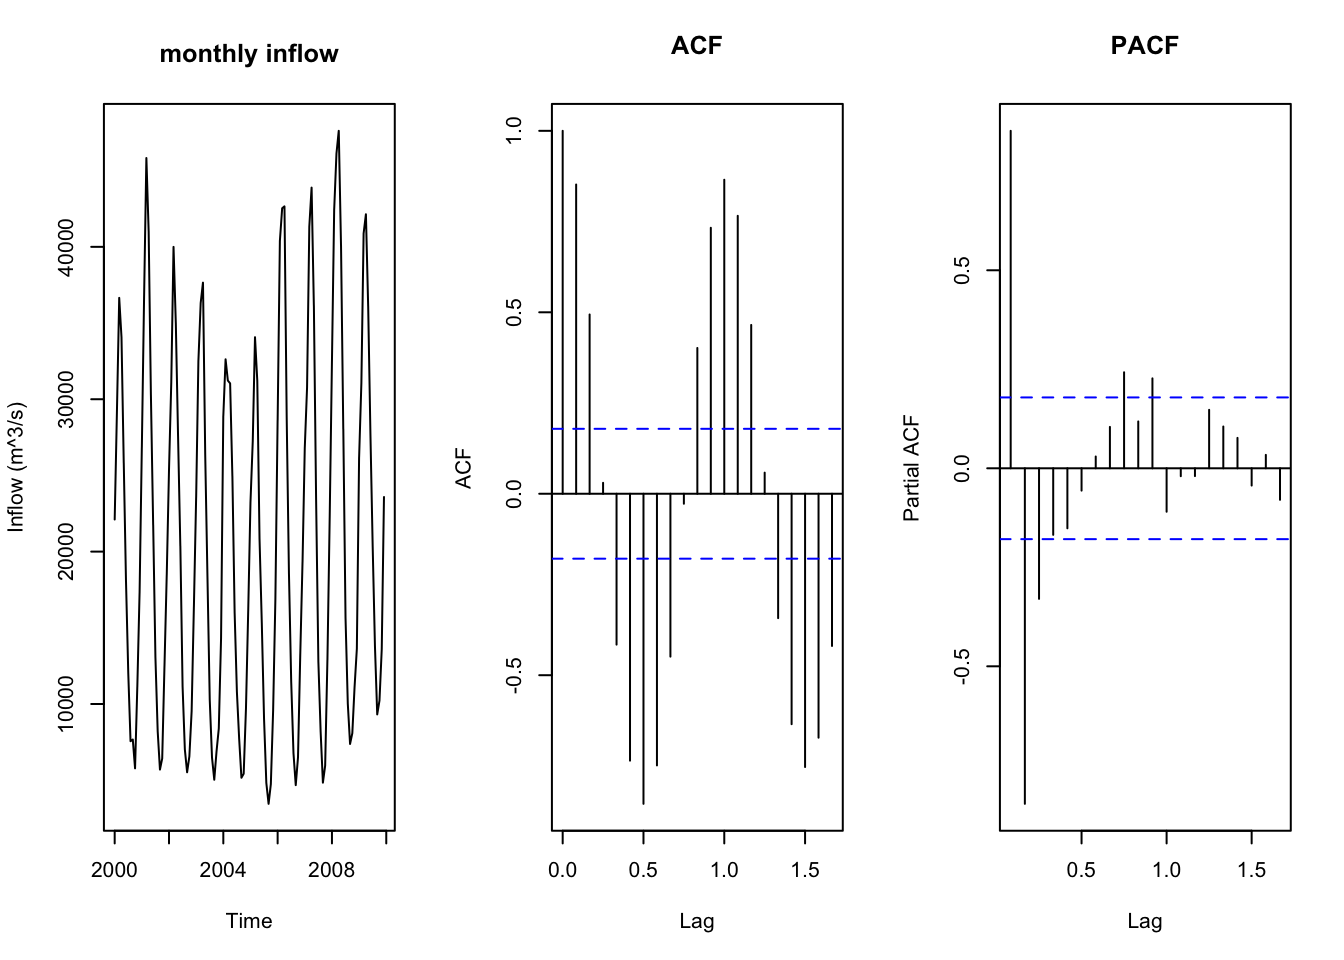
\includegraphics{YuxiangRen_TSA_A03_Sp23_files/figure-latex/Q1-1.pdf}

\begin{Shaded}
\begin{Highlighting}[]
\CommentTok{\# Total Renewable Energy Production}
\FunctionTok{par}\NormalTok{(}\AttributeTok{mfrow =} \FunctionTok{c}\NormalTok{(}\DecValTok{1}\NormalTok{, }\DecValTok{3}\NormalTok{))}
\FunctionTok{plot}\NormalTok{(}\AttributeTok{x =}\NormalTok{ rawdata}\SpecialCharTok{$}\NormalTok{Month, }\AttributeTok{y =}\NormalTok{ rawdata}\SpecialCharTok{$}\StringTok{\textasciigrave{}}\AttributeTok{Total Renewable Energy Production}\StringTok{\textasciigrave{}}\NormalTok{, }\AttributeTok{type =} \StringTok{"l"}\NormalTok{,}
    \AttributeTok{xlab =} \StringTok{"Year"}\NormalTok{, }\AttributeTok{ylab =} \StringTok{"Energy Production (Trillion Btu)"}\NormalTok{, }\AttributeTok{main =} \StringTok{"Time series plot"}\NormalTok{)}
\FunctionTok{Acf}\NormalTok{(ts\_A03[, }\StringTok{"Total Renewable Energy Production"}\NormalTok{], }\AttributeTok{lag.max =} \DecValTok{40}\NormalTok{, }\AttributeTok{main =} \FunctionTok{paste}\NormalTok{(}\StringTok{"Total Renewable Energy Production"}\NormalTok{))}
\FunctionTok{Pacf}\NormalTok{(ts\_A03[, }\StringTok{"Total Renewable Energy Production"}\NormalTok{], }\AttributeTok{lag.max =} \DecValTok{40}\NormalTok{, }\AttributeTok{main =} \FunctionTok{paste}\NormalTok{(}\StringTok{""}\NormalTok{))}
\end{Highlighting}
\end{Shaded}

\includegraphics{YuxiangRen_TSA_A03_Sp23_files/figure-latex/Q1-2.pdf}

\begin{Shaded}
\begin{Highlighting}[]
\CommentTok{\# Hydroelectric Power Consumption}
\FunctionTok{par}\NormalTok{(}\AttributeTok{mfrow =} \FunctionTok{c}\NormalTok{(}\DecValTok{1}\NormalTok{, }\DecValTok{3}\NormalTok{))}
\FunctionTok{plot}\NormalTok{(}\AttributeTok{x =}\NormalTok{ rawdata}\SpecialCharTok{$}\NormalTok{Month, }\AttributeTok{y =}\NormalTok{ rawdata}\SpecialCharTok{$}\StringTok{\textasciigrave{}}\AttributeTok{Hydroelectric Power Consumption}\StringTok{\textasciigrave{}}\NormalTok{, }\AttributeTok{type =} \StringTok{"l"}\NormalTok{,}
    \AttributeTok{xlab =} \StringTok{"Year"}\NormalTok{, }\AttributeTok{ylab =} \StringTok{"Energy Consumption (Trillion Btu)"}\NormalTok{, }\AttributeTok{main =} \StringTok{"Time series plot"}\NormalTok{)}
\FunctionTok{Acf}\NormalTok{(ts\_A03[, }\StringTok{"Hydroelectric Power Consumption"}\NormalTok{], }\AttributeTok{lag.max =} \DecValTok{40}\NormalTok{, }\AttributeTok{main =} \FunctionTok{paste}\NormalTok{(}\StringTok{"Hydroelectric Power Consumption"}\NormalTok{))}
\FunctionTok{Pacf}\NormalTok{(ts\_A03[, }\StringTok{"Hydroelectric Power Consumption"}\NormalTok{], }\AttributeTok{lag.max =} \DecValTok{40}\NormalTok{, }\AttributeTok{main =} \FunctionTok{paste}\NormalTok{(}\StringTok{""}\NormalTok{))}
\end{Highlighting}
\end{Shaded}

\includegraphics{YuxiangRen_TSA_A03_Sp23_files/figure-latex/Q1-3.pdf}

\hypertarget{q2}{%
\subsubsection{Q2}\label{q2}}

From the plot in Q1, do the series Total Biomass Energy Production,
Total Renewable Energy Production, Hydroelectric Power Consumption
appear to have a trend? If yes, what kind of trend?

\begin{quote}
Answer: They have trends. For Total Biomass Energy Production and Total
Renewable Energy Production, there is a gradual upward trend. For
Hydroelectric Power Consumption, the overall trend is downward.
\end{quote}

\hypertarget{q3}{%
\subsubsection{Q3}\label{q3}}

Use the \emph{lm()} function to fit a linear trend to the three time
series. Ask R to print the summary of the regression. Interpret the
regression output, i.e., slope and intercept. Save the regression
coefficients for further analysis.

\begin{Shaded}
\begin{Highlighting}[]
\NormalTok{t }\OtherTok{\textless{}{-}} \FunctionTok{c}\NormalTok{(}\DecValTok{1}\SpecialCharTok{:}\NormalTok{nrow)}
\CommentTok{\# Total Biomass Energy Production}
\NormalTok{bio\_linear\_trend }\OtherTok{=} \FunctionTok{lm}\NormalTok{(rawdata}\SpecialCharTok{$}\StringTok{\textasciigrave{}}\AttributeTok{Total Biomass Energy Production}\StringTok{\textasciigrave{}} \SpecialCharTok{\textasciitilde{}}\NormalTok{ t)}
\NormalTok{bio\_beta0 }\OtherTok{=} \FunctionTok{as.numeric}\NormalTok{(bio\_linear\_trend}\SpecialCharTok{$}\NormalTok{coefficients[}\DecValTok{1}\NormalTok{])  }\CommentTok{\#intercept}
\NormalTok{bio\_beta1 }\OtherTok{=} \FunctionTok{as.numeric}\NormalTok{(bio\_linear\_trend}\SpecialCharTok{$}\NormalTok{coefficients[}\DecValTok{2}\NormalTok{])  }\CommentTok{\#slope}
\FunctionTok{summary}\NormalTok{(bio\_linear\_trend)}
\end{Highlighting}
\end{Shaded}

\begin{verbatim}
## 
## Call:
## lm(formula = rawdata$`Total Biomass Energy Production` ~ t)
## 
## Residuals:
##      Min       1Q   Median       3Q      Max 
## -102.800  -23.994    5.667   32.265   82.192 
## 
## Coefficients:
##              Estimate Std. Error t value Pr(>|t|)    
## (Intercept) 1.337e+02  3.245e+00   41.22   <2e-16 ***
## t           4.800e-01  9.402e-03   51.05   <2e-16 ***
## ---
## Signif. codes:  0 '***' 0.001 '**' 0.01 '*' 0.05 '.' 0.1 ' ' 1
## 
## Residual standard error: 39.59 on 595 degrees of freedom
## Multiple R-squared:  0.8142, Adjusted R-squared:  0.8138 
## F-statistic:  2607 on 1 and 595 DF,  p-value: < 2.2e-16
\end{verbatim}

\begin{Shaded}
\begin{Highlighting}[]
\CommentTok{\# Total Renewable Energy Production}
\NormalTok{ren\_linear\_trend }\OtherTok{=} \FunctionTok{lm}\NormalTok{(rawdata[, }\StringTok{"Total Renewable Energy Production"}\NormalTok{] }\SpecialCharTok{\textasciitilde{}}\NormalTok{ t)}
\NormalTok{ren\_beta0 }\OtherTok{=} \FunctionTok{as.numeric}\NormalTok{(ren\_linear\_trend}\SpecialCharTok{$}\NormalTok{coefficients[}\DecValTok{1}\NormalTok{])  }\CommentTok{\#intercept}
\NormalTok{ren\_beta1 }\OtherTok{=} \FunctionTok{as.numeric}\NormalTok{(ren\_linear\_trend}\SpecialCharTok{$}\NormalTok{coefficients[}\DecValTok{2}\NormalTok{])  }\CommentTok{\#slope}
\FunctionTok{summary}\NormalTok{(ren\_linear\_trend)}
\end{Highlighting}
\end{Shaded}

\begin{verbatim}
## 
## Call:
## lm(formula = rawdata[, "Total Renewable Energy Production"] ~ 
##     t)
## 
## Residuals:
##     Min      1Q  Median      3Q     Max 
## -238.75  -61.85    8.59   64.48  352.27 
## 
## Coefficients:
##             Estimate Std. Error t value Pr(>|t|)    
## (Intercept) 312.2475     8.4902   36.78   <2e-16 ***
## t             0.9362     0.0246   38.05   <2e-16 ***
## ---
## Signif. codes:  0 '***' 0.001 '**' 0.01 '*' 0.05 '.' 0.1 ' ' 1
## 
## Residual standard error: 103.6 on 595 degrees of freedom
## Multiple R-squared:  0.7088, Adjusted R-squared:  0.7083 
## F-statistic:  1448 on 1 and 595 DF,  p-value: < 2.2e-16
\end{verbatim}

\begin{Shaded}
\begin{Highlighting}[]
\CommentTok{\# Hydroelectric Power Consumption}
\NormalTok{hyd\_linear\_trend }\OtherTok{=} \FunctionTok{lm}\NormalTok{(rawdata[, }\StringTok{"Hydroelectric Power Consumption"}\NormalTok{] }\SpecialCharTok{\textasciitilde{}}\NormalTok{ t)}
\NormalTok{hyd\_beta0 }\OtherTok{=} \FunctionTok{as.numeric}\NormalTok{(hyd\_linear\_trend}\SpecialCharTok{$}\NormalTok{coefficients[}\DecValTok{1}\NormalTok{])  }\CommentTok{\#intercept}
\NormalTok{hyd\_beta1 }\OtherTok{=} \FunctionTok{as.numeric}\NormalTok{(hyd\_linear\_trend}\SpecialCharTok{$}\NormalTok{coefficients[}\DecValTok{2}\NormalTok{])  }\CommentTok{\#slope}
\FunctionTok{summary}\NormalTok{(hyd\_linear\_trend)}
\end{Highlighting}
\end{Shaded}

\begin{verbatim}
## 
## Call:
## lm(formula = rawdata[, "Hydroelectric Power Consumption"] ~ t)
## 
## Residuals:
##    Min     1Q Median     3Q    Max 
## -95.42 -31.20  -2.56  27.32 121.61 
## 
## Coefficients:
##               Estimate Std. Error t value Pr(>|t|)    
## (Intercept) 259.898013   3.427300  75.832  < 2e-16 ***
## t            -0.082888   0.009931  -8.346 4.94e-16 ***
## ---
## Signif. codes:  0 '***' 0.001 '**' 0.01 '*' 0.05 '.' 0.1 ' ' 1
## 
## Residual standard error: 41.82 on 595 degrees of freedom
## Multiple R-squared:  0.1048, Adjusted R-squared:  0.1033 
## F-statistic: 69.66 on 1 and 595 DF,  p-value: 4.937e-16
\end{verbatim}

\begin{quote}
Answer:For Total Biomass Energy Production' linear trend, the intercept
is 133.74, and slope is 0.48. For Total Renewable Energy Production's
linear trend, the intercept is 312.25, and slope is 0.94. For
Hydroelectric Power Consumption's linear trend, the intercept is 259.90
and slope is -0.08
\end{quote}

\hypertarget{q4}{%
\subsubsection{Q4}\label{q4}}

Use the regression coefficients from Q3 to detrend the series. Plot the
detrended series and compare with the plots from Q1. What happened? Did
anything change?

\begin{Shaded}
\begin{Highlighting}[]
\CommentTok{\# Total Biomass Energy Production}
\NormalTok{bio\_detrend }\OtherTok{\textless{}{-}}\NormalTok{ rawdata}\SpecialCharTok{$}\StringTok{\textasciigrave{}}\AttributeTok{Total Biomass Energy Production}\StringTok{\textasciigrave{}} \SpecialCharTok{{-}}\NormalTok{ (bio\_beta0 }\SpecialCharTok{+}\NormalTok{ bio\_beta1 }\SpecialCharTok{*}
\NormalTok{    t)}
\FunctionTok{ggplot}\NormalTok{(rawdata, }\FunctionTok{aes}\NormalTok{(}\AttributeTok{x =}\NormalTok{ Month, }\AttributeTok{y =} \StringTok{\textasciigrave{}}\AttributeTok{Total Biomass Energy Production}\StringTok{\textasciigrave{}}\NormalTok{)) }\SpecialCharTok{+} \FunctionTok{geom\_line}\NormalTok{(}\AttributeTok{color =} \StringTok{"black"}\NormalTok{) }\SpecialCharTok{+}
    \FunctionTok{geom\_line}\NormalTok{(}\FunctionTok{aes}\NormalTok{(}\AttributeTok{y =}\NormalTok{ bio\_detrend), }\AttributeTok{col =} \StringTok{"green"}\NormalTok{) }\SpecialCharTok{+} \FunctionTok{ggtitle}\NormalTok{(}\StringTok{"Total Biomass Energy Production"}\NormalTok{) }\SpecialCharTok{+}
    \FunctionTok{xlab}\NormalTok{(}\StringTok{"Year"}\NormalTok{) }\SpecialCharTok{+} \FunctionTok{ylab}\NormalTok{(}\StringTok{"Energy Production (Trillion Btu)"}\NormalTok{)}
\end{Highlighting}
\end{Shaded}

\includegraphics{YuxiangRen_TSA_A03_Sp23_files/figure-latex/Q4 detrend-1.pdf}

\begin{Shaded}
\begin{Highlighting}[]
\CommentTok{\# Total Renewable Energy Production}
\NormalTok{ren\_detrend }\OtherTok{\textless{}{-}}\NormalTok{ rawdata}\SpecialCharTok{$}\StringTok{\textasciigrave{}}\AttributeTok{Total Renewable Energy Production}\StringTok{\textasciigrave{}} \SpecialCharTok{{-}}\NormalTok{ (ren\_beta0 }\SpecialCharTok{+}\NormalTok{ ren\_beta1 }\SpecialCharTok{*}
\NormalTok{    t)}
\FunctionTok{ggplot}\NormalTok{(rawdata, }\FunctionTok{aes}\NormalTok{(}\AttributeTok{x =}\NormalTok{ Month, }\AttributeTok{y =} \StringTok{\textasciigrave{}}\AttributeTok{Total Renewable Energy Production}\StringTok{\textasciigrave{}}\NormalTok{)) }\SpecialCharTok{+} \FunctionTok{geom\_line}\NormalTok{(}\AttributeTok{color =} \StringTok{"black"}\NormalTok{) }\SpecialCharTok{+}
    \FunctionTok{geom\_line}\NormalTok{(}\FunctionTok{aes}\NormalTok{(}\AttributeTok{y =}\NormalTok{ ren\_detrend), }\AttributeTok{col =} \StringTok{"green"}\NormalTok{) }\SpecialCharTok{+} \FunctionTok{ggtitle}\NormalTok{(}\StringTok{"Total Renewable Energy Production"}\NormalTok{) }\SpecialCharTok{+}
    \FunctionTok{xlab}\NormalTok{(}\StringTok{"Year"}\NormalTok{) }\SpecialCharTok{+} \FunctionTok{ylab}\NormalTok{(}\StringTok{"Energy Production (Trillion Btu)"}\NormalTok{)}
\end{Highlighting}
\end{Shaded}

\includegraphics{YuxiangRen_TSA_A03_Sp23_files/figure-latex/Q4 detrend-2.pdf}

\begin{Shaded}
\begin{Highlighting}[]
\CommentTok{\# Hydroelectric Power Consumption}
\NormalTok{hyd\_detrend }\OtherTok{\textless{}{-}}\NormalTok{ rawdata}\SpecialCharTok{$}\StringTok{\textasciigrave{}}\AttributeTok{Hydroelectric Power Consumption}\StringTok{\textasciigrave{}} \SpecialCharTok{{-}}\NormalTok{ (hyd\_beta0 }\SpecialCharTok{+}\NormalTok{ hyd\_beta1 }\SpecialCharTok{*}
\NormalTok{    t)}
\FunctionTok{ggplot}\NormalTok{(rawdata, }\FunctionTok{aes}\NormalTok{(}\AttributeTok{x =}\NormalTok{ Month, }\AttributeTok{y =} \StringTok{\textasciigrave{}}\AttributeTok{Hydroelectric Power Consumption}\StringTok{\textasciigrave{}}\NormalTok{)) }\SpecialCharTok{+} \FunctionTok{geom\_line}\NormalTok{(}\AttributeTok{color =} \StringTok{"black"}\NormalTok{) }\SpecialCharTok{+}
    \FunctionTok{geom\_line}\NormalTok{(}\FunctionTok{aes}\NormalTok{(}\AttributeTok{y =}\NormalTok{ hyd\_detrend), }\AttributeTok{col =} \StringTok{"green"}\NormalTok{) }\SpecialCharTok{+} \FunctionTok{ggtitle}\NormalTok{(}\StringTok{"Hydroelectric Power Consumption"}\NormalTok{) }\SpecialCharTok{+}
    \FunctionTok{xlab}\NormalTok{(}\StringTok{"Year"}\NormalTok{) }\SpecialCharTok{+} \FunctionTok{ylab}\NormalTok{(}\StringTok{"Energy Consumption (Trillion Btu)"}\NormalTok{)}
\end{Highlighting}
\end{Shaded}

\includegraphics{YuxiangRen_TSA_A03_Sp23_files/figure-latex/Q4 detrend-3.pdf}

\begin{quote}
Answer: In the above three Figures, the black lines are the original
data, and the greens are the detrended data. It can be seen that all the
data have been shifted down, and their value range is close to 0. For
the Total Biomass Energy Production and Total Renewable Energy
Production, the growth rate in detrend data are reduced, and there
emerge several downward trends compared with the original data. For
Hydroelectric Power Consumption, the original downward trend is barely
detectable.
\end{quote}

\hypertarget{q5}{%
\subsubsection{Q5}\label{q5}}

Plot ACF and PACF for the detrended series and compare with the plots
from Q1. Did the plots change? How?

\begin{Shaded}
\begin{Highlighting}[]
\CommentTok{\# Total Biomass Energy Production}
\NormalTok{ts\_detrendBio }\OtherTok{\textless{}{-}} \FunctionTok{ts}\NormalTok{(bio\_detrend, }\AttributeTok{frequency =} \DecValTok{12}\NormalTok{, }\AttributeTok{start =} \FunctionTok{c}\NormalTok{(}\DecValTok{1973}\NormalTok{, }\DecValTok{1}\NormalTok{))}
\FunctionTok{par}\NormalTok{(}\AttributeTok{mfrow =} \FunctionTok{c}\NormalTok{(}\DecValTok{2}\NormalTok{, }\DecValTok{2}\NormalTok{))}
\FunctionTok{Acf}\NormalTok{(ts\_A03[, }\StringTok{"Total Biomass Energy Production"}\NormalTok{], }\AttributeTok{lag.max =} \DecValTok{40}\NormalTok{, }\AttributeTok{main =} \FunctionTok{paste}\NormalTok{(}\StringTok{"Biomass Original"}\NormalTok{))}
\FunctionTok{Pacf}\NormalTok{(ts\_A03[, }\StringTok{"Total Biomass Energy Production"}\NormalTok{], }\AttributeTok{lag.max =} \DecValTok{40}\NormalTok{, }\AttributeTok{main =} \FunctionTok{paste}\NormalTok{(}\StringTok{"Original"}\NormalTok{))}
\FunctionTok{Acf}\NormalTok{(ts\_detrendBio, }\AttributeTok{lag.max =} \DecValTok{40}\NormalTok{, }\AttributeTok{main =} \FunctionTok{paste}\NormalTok{(}\StringTok{"Detrend"}\NormalTok{))}
\FunctionTok{Pacf}\NormalTok{(ts\_detrendBio, }\AttributeTok{lag.max =} \DecValTok{40}\NormalTok{, }\AttributeTok{main =} \FunctionTok{paste}\NormalTok{(}\StringTok{"Detrend"}\NormalTok{))}
\end{Highlighting}
\end{Shaded}

\includegraphics{YuxiangRen_TSA_A03_Sp23_files/figure-latex/Q5-1.pdf}

\begin{Shaded}
\begin{Highlighting}[]
\CommentTok{\# Total Renewable Energy Production}
\NormalTok{ts\_detrendRen }\OtherTok{\textless{}{-}} \FunctionTok{ts}\NormalTok{(ren\_detrend, }\AttributeTok{frequency =} \DecValTok{12}\NormalTok{, }\AttributeTok{start =} \FunctionTok{c}\NormalTok{(}\DecValTok{1973}\NormalTok{, }\DecValTok{1}\NormalTok{))}
\FunctionTok{par}\NormalTok{(}\AttributeTok{mfrow =} \FunctionTok{c}\NormalTok{(}\DecValTok{2}\NormalTok{, }\DecValTok{2}\NormalTok{))}
\FunctionTok{Acf}\NormalTok{(ts\_A03[, }\StringTok{"Total Renewable Energy Production"}\NormalTok{], }\AttributeTok{lag.max =} \DecValTok{40}\NormalTok{, }\AttributeTok{main =} \FunctionTok{paste}\NormalTok{(}\StringTok{"Renewable Original"}\NormalTok{))}
\FunctionTok{Pacf}\NormalTok{(ts\_A03[, }\StringTok{"Total Renewable Energy Production"}\NormalTok{], }\AttributeTok{lag.max =} \DecValTok{40}\NormalTok{, }\AttributeTok{main =} \FunctionTok{paste}\NormalTok{(}\StringTok{"Original"}\NormalTok{))}
\FunctionTok{Acf}\NormalTok{(ts\_detrendRen, }\AttributeTok{lag.max =} \DecValTok{40}\NormalTok{, }\AttributeTok{main =} \FunctionTok{paste}\NormalTok{(}\StringTok{"Detrend"}\NormalTok{))}
\FunctionTok{Pacf}\NormalTok{(ts\_detrendRen, }\AttributeTok{lag.max =} \DecValTok{40}\NormalTok{, }\AttributeTok{main =} \FunctionTok{paste}\NormalTok{(}\StringTok{"Detrend"}\NormalTok{))}
\end{Highlighting}
\end{Shaded}

\includegraphics{YuxiangRen_TSA_A03_Sp23_files/figure-latex/Q5-2.pdf}

\begin{Shaded}
\begin{Highlighting}[]
\CommentTok{\# Hydroelectric Power Consumption}
\NormalTok{ts\_detrendHyd }\OtherTok{\textless{}{-}} \FunctionTok{ts}\NormalTok{(hyd\_detrend, }\AttributeTok{frequency =} \DecValTok{12}\NormalTok{, }\AttributeTok{start =} \FunctionTok{c}\NormalTok{(}\DecValTok{1973}\NormalTok{, }\DecValTok{1}\NormalTok{))}
\FunctionTok{par}\NormalTok{(}\AttributeTok{mfrow =} \FunctionTok{c}\NormalTok{(}\DecValTok{2}\NormalTok{, }\DecValTok{2}\NormalTok{))}
\FunctionTok{Acf}\NormalTok{(ts\_A03[, }\StringTok{"Hydroelectric Power Consumption"}\NormalTok{], }\AttributeTok{lag.max =} \DecValTok{40}\NormalTok{, }\AttributeTok{main =} \FunctionTok{paste}\NormalTok{(}\StringTok{"Hydroelectric Original"}\NormalTok{))}
\FunctionTok{Pacf}\NormalTok{(ts\_A03[, }\StringTok{"Hydroelectric Power Consumption"}\NormalTok{], }\AttributeTok{lag.max =} \DecValTok{40}\NormalTok{, }\AttributeTok{main =} \FunctionTok{paste}\NormalTok{(}\StringTok{"Original"}\NormalTok{))}
\FunctionTok{Acf}\NormalTok{(ts\_detrendHyd, }\AttributeTok{lag.max =} \DecValTok{40}\NormalTok{, }\AttributeTok{main =} \FunctionTok{paste}\NormalTok{(}\StringTok{"Detrend"}\NormalTok{))}
\FunctionTok{Pacf}\NormalTok{(ts\_detrendHyd, }\AttributeTok{lag.max =} \DecValTok{40}\NormalTok{, }\AttributeTok{main =} \FunctionTok{paste}\NormalTok{(}\StringTok{"Detrend"}\NormalTok{))}
\end{Highlighting}
\end{Shaded}

\includegraphics{YuxiangRen_TSA_A03_Sp23_files/figure-latex/Q5-3.pdf}

\begin{quote}
Answer: Plots change. For Total Biomass Energy Production and Total
Renewable Energy Production, the value of autocorrelation in the detrend
ACF graph is no longer a simple gradual decrease, which is accompanied
by obvious periodical fluctuations. The values in detrend ACF at 12, 24,
and 36 lag points become larger, making the difference with nearby lags
more obvious. Additionally, in PACF, there are more lag values
increasing, especially at lags 12, 24, and 36. For Hydroelectric Power
Consumption, the autocorrelation of many lag points with negative values
in ACF has been strengthened.
\end{quote}

\hypertarget{seasonal-component}{%
\subsection{Seasonal Component}\label{seasonal-component}}

Set aside the detrended series and consider the original series again
from Q1 to answer Q6 to Q8.

\hypertarget{q6}{%
\subsubsection{Q6}\label{q6}}

Do the series seem to have a seasonal trend? Which serie/series? Use
function \emph{lm()} to fit a seasonal means model (i.e.~using the
seasonal dummies) to this/these time series. Ask R to print the summary
of the regression. Interpret the regression output. Save the regression
coefficients for further analysis.

\begin{Shaded}
\begin{Highlighting}[]
\CommentTok{\# Total Biomass Energy Production}
\NormalTok{bio\_dummies }\OtherTok{\textless{}{-}} \FunctionTok{seasonaldummy}\NormalTok{(ts\_A03[, }\DecValTok{1}\NormalTok{])}
\DocumentationTok{\#\# Then fit a linear model to the seasonal dummies}
\NormalTok{bio\_seas\_means\_model }\OtherTok{=} \FunctionTok{lm}\NormalTok{(rawdata}\SpecialCharTok{$}\StringTok{\textasciigrave{}}\AttributeTok{Total Biomass Energy Production}\StringTok{\textasciigrave{}} \SpecialCharTok{\textasciitilde{}}\NormalTok{ bio\_dummies)}
\FunctionTok{print}\NormalTok{(}\FunctionTok{summary}\NormalTok{(bio\_seas\_means\_model))}
\end{Highlighting}
\end{Shaded}

\begin{verbatim}
## 
## Call:
## lm(formula = rawdata$`Total Biomass Energy Production` ~ bio_dummies)
## 
## Residuals:
##     Min      1Q  Median      3Q     Max 
## -160.74  -53.67  -24.36   90.73  181.34 
## 
## Coefficients:
##                Estimate Std. Error t value Pr(>|t|)    
## (Intercept)     288.020     13.163  21.881   <2e-16 ***
## bio_dummiesJan   -1.793     18.522  -0.097   0.9229    
## bio_dummiesFeb  -31.102     18.522  -1.679   0.0936 .  
## bio_dummiesMar   -9.104     18.522  -0.492   0.6232    
## bio_dummiesApr  -21.502     18.522  -1.161   0.2462    
## bio_dummiesMay  -14.238     18.522  -0.769   0.4424    
## bio_dummiesJun  -19.602     18.522  -1.058   0.2904    
## bio_dummiesJul   -3.674     18.522  -0.198   0.8428    
## bio_dummiesAug   -0.612     18.522  -0.033   0.9737    
## bio_dummiesSep  -13.335     18.522  -0.720   0.4718    
## bio_dummiesOct   -4.030     18.615  -0.216   0.8287    
## bio_dummiesNov   -9.849     18.615  -0.529   0.5970    
## ---
## Signif. codes:  0 '***' 0.001 '**' 0.01 '*' 0.05 '.' 0.1 ' ' 1
## 
## Residual standard error: 92.14 on 585 degrees of freedom
## Multiple R-squared:  0.01018,    Adjusted R-squared:  -0.008437 
## F-statistic: 0.5467 on 11 and 585 DF,  p-value: 0.8714
\end{verbatim}

\begin{Shaded}
\begin{Highlighting}[]
\DocumentationTok{\#\# Store regression coefficients}
\NormalTok{bio\_season\_beta\_int }\OtherTok{=}\NormalTok{ bio\_seas\_means\_model}\SpecialCharTok{$}\NormalTok{coefficients[}\DecValTok{1}\NormalTok{]}
\NormalTok{bio\_season\_beta\_coeff }\OtherTok{=}\NormalTok{ bio\_seas\_means\_model}\SpecialCharTok{$}\NormalTok{coefficients[}\DecValTok{2}\SpecialCharTok{:}\DecValTok{12}\NormalTok{]}

\CommentTok{\# Total Renewable Energy Production}
\NormalTok{ren\_dummies }\OtherTok{\textless{}{-}} \FunctionTok{seasonaldummy}\NormalTok{(ts\_A03[, }\DecValTok{2}\NormalTok{])}
\DocumentationTok{\#\# Then fit a linear model to the seasonal dummies}
\NormalTok{ren\_seas\_means\_model }\OtherTok{=} \FunctionTok{lm}\NormalTok{(rawdata}\SpecialCharTok{$}\StringTok{\textasciigrave{}}\AttributeTok{Total Renewable Energy Production}\StringTok{\textasciigrave{}} \SpecialCharTok{\textasciitilde{}}\NormalTok{ ren\_dummies)}
\FunctionTok{print}\NormalTok{(}\FunctionTok{summary}\NormalTok{(ren\_seas\_means\_model))}
\end{Highlighting}
\end{Shaded}

\begin{verbatim}
## 
## Call:
## lm(formula = rawdata$`Total Renewable Energy Production` ~ ren_dummies)
## 
## Residuals:
##     Min      1Q  Median      3Q     Max 
## -284.92 -122.23  -68.42   91.22  585.68 
## 
## Coefficients:
##                Estimate Std. Error t value Pr(>|t|)    
## (Intercept)     601.022     27.260  22.048   <2e-16 ***
## ren_dummiesJan   11.468     38.358   0.299    0.765    
## ren_dummiesFeb  -41.456     38.358  -1.081    0.280    
## ren_dummiesMar   23.130     38.358   0.603    0.547    
## ren_dummiesApr    9.959     38.358   0.260    0.795    
## ren_dummiesMay   38.853     38.358   1.013    0.312    
## ren_dummiesJun   20.378     38.358   0.531    0.595    
## ren_dummiesJul    8.298     38.358   0.216    0.829    
## ren_dummiesAug  -19.450     38.358  -0.507    0.612    
## ren_dummiesSep  -63.770     38.358  -1.662    0.097 .  
## ren_dummiesOct  -52.612     38.551  -1.365    0.173    
## ren_dummiesNov  -42.537     38.551  -1.103    0.270    
## ---
## Signif. codes:  0 '***' 0.001 '**' 0.01 '*' 0.05 '.' 0.1 ' ' 1
## 
## Residual standard error: 190.8 on 585 degrees of freedom
## Multiple R-squared:  0.02844,    Adjusted R-squared:  0.01017 
## F-statistic: 1.557 on 11 and 585 DF,  p-value: 0.1076
\end{verbatim}

\begin{Shaded}
\begin{Highlighting}[]
\DocumentationTok{\#\# Store regression coefficients}
\NormalTok{ren\_season\_beta\_int }\OtherTok{=}\NormalTok{ ren\_seas\_means\_model}\SpecialCharTok{$}\NormalTok{coefficients[}\DecValTok{1}\NormalTok{]}
\NormalTok{ren\_season\_beta\_coeff }\OtherTok{=}\NormalTok{ ren\_seas\_means\_model}\SpecialCharTok{$}\NormalTok{coefficients[}\DecValTok{2}\SpecialCharTok{:}\DecValTok{12}\NormalTok{]}

\CommentTok{\# Hydroelectric Power Consumption}
\NormalTok{hyd\_dummies }\OtherTok{\textless{}{-}} \FunctionTok{seasonaldummy}\NormalTok{(ts\_A03[, }\DecValTok{3}\NormalTok{])}
\DocumentationTok{\#\# Then fit a linear model to the seasonal dummies}
\NormalTok{hyd\_seas\_means\_model }\OtherTok{=} \FunctionTok{lm}\NormalTok{(rawdata}\SpecialCharTok{$}\StringTok{\textasciigrave{}}\AttributeTok{Hydroelectric Power Consumption}\StringTok{\textasciigrave{}} \SpecialCharTok{\textasciitilde{}}\NormalTok{ hyd\_dummies)}
\FunctionTok{print}\NormalTok{(}\FunctionTok{summary}\NormalTok{(hyd\_seas\_means\_model))}
\end{Highlighting}
\end{Shaded}

\begin{verbatim}
## 
## Call:
## lm(formula = rawdata$`Hydroelectric Power Consumption` ~ hyd_dummies)
## 
## Residuals:
##    Min     1Q Median     3Q    Max 
## -88.99 -23.47  -2.81  21.99 100.18 
## 
## Coefficients:
##                Estimate Std. Error t value Pr(>|t|)    
## (Intercept)     237.225      4.878  48.634  < 2e-16 ***
## hyd_dummiesJan   13.594      6.864   1.981  0.04811 *  
## hyd_dummiesFeb   -8.254      6.864  -1.203  0.22964    
## hyd_dummiesMar   19.980      6.864   2.911  0.00374 ** 
## hyd_dummiesApr   15.649      6.864   2.280  0.02297 *  
## hyd_dummiesMay   39.210      6.864   5.713 1.77e-08 ***
## hyd_dummiesJun   31.209      6.864   4.547 6.61e-06 ***
## hyd_dummiesJul   10.436      6.864   1.520  0.12895    
## hyd_dummiesAug  -17.909      6.864  -2.609  0.00931 ** 
## hyd_dummiesSep  -50.173      6.864  -7.310 8.82e-13 ***
## hyd_dummiesOct  -48.262      6.898  -6.996 7.22e-12 ***
## hyd_dummiesNov  -32.285      6.898  -4.680 3.56e-06 ***
## ---
## Signif. codes:  0 '***' 0.001 '**' 0.01 '*' 0.05 '.' 0.1 ' ' 1
## 
## Residual standard error: 34.14 on 585 degrees of freedom
## Multiple R-squared:  0.4132, Adjusted R-squared:  0.4022 
## F-statistic: 37.45 on 11 and 585 DF,  p-value: < 2.2e-16
\end{verbatim}

\begin{Shaded}
\begin{Highlighting}[]
\DocumentationTok{\#\# Store regression coefficients}
\NormalTok{hyd\_season\_beta\_int }\OtherTok{=}\NormalTok{ hyd\_seas\_means\_model}\SpecialCharTok{$}\NormalTok{coefficients[}\DecValTok{1}\NormalTok{]}
\NormalTok{hyd\_season\_beta\_coeff }\OtherTok{=}\NormalTok{ hyd\_seas\_means\_model}\SpecialCharTok{$}\NormalTok{coefficients[}\DecValTok{2}\SpecialCharTok{:}\DecValTok{12}\NormalTok{]}
\end{Highlighting}
\end{Shaded}

\begin{quote}
Answer: For both Total Biomass Energy Production and Total Renewable
Energy Production, most coefficients are negative. Meanwhile, due to
higher p values, all regression results are not statistically
significant. For Hydroelectric Power Consumption, most of the seasonal
dummies have p-values less than 0.05, including Jan, Mar, Apr, May, Jun,
Aug, Sep, Oct, and Nov, indicating a significant relationship between
the time series and those seasons. More specifically, coefficients are
positive in Mar, Apr, May and Jun, while the coefficients are negative
in Aug, Sep, Oct and Nov.~Therefore, only Hydroelectric Power
Consumption data seem to have seasonal trend.
\end{quote}

\hypertarget{q7}{%
\subsubsection{Q7}\label{q7}}

Use the regression coefficients from Q6 to deseason the series. Plot the
deseason series and compare with the plots from part Q1. Did anything
change?

\begin{Shaded}
\begin{Highlighting}[]
\CommentTok{\# Total Biomass Energy Production compute seasonal component}
\NormalTok{bio\_seas\_comp }\OtherTok{=} \FunctionTok{array}\NormalTok{(}\DecValTok{0}\NormalTok{, nrow)}
\ControlFlowTok{for}\NormalTok{ (i }\ControlFlowTok{in} \DecValTok{1}\SpecialCharTok{:}\NormalTok{nrow) \{}
\NormalTok{    bio\_seas\_comp[i] }\OtherTok{=}\NormalTok{ (bio\_season\_beta\_int }\SpecialCharTok{+}\NormalTok{ bio\_season\_beta\_coeff }\SpecialCharTok{\%*\%}\NormalTok{ bio\_dummies[i,}
\NormalTok{        ])}
\NormalTok{\}}
\DocumentationTok{\#\# deseason}
\NormalTok{bio\_deseason }\OtherTok{\textless{}{-}}\NormalTok{ rawdata}\SpecialCharTok{$}\StringTok{\textasciigrave{}}\AttributeTok{Total Biomass Energy Production}\StringTok{\textasciigrave{}} \SpecialCharTok{{-}}\NormalTok{ bio\_seas\_comp}
\FunctionTok{ggplot}\NormalTok{(rawdata, }\FunctionTok{aes}\NormalTok{(}\AttributeTok{x =}\NormalTok{ Month, }\AttributeTok{y =} \StringTok{\textasciigrave{}}\AttributeTok{Total Biomass Energy Production}\StringTok{\textasciigrave{}}\NormalTok{)) }\SpecialCharTok{+} \FunctionTok{geom\_line}\NormalTok{(}\AttributeTok{color =} \StringTok{"black"}\NormalTok{) }\SpecialCharTok{+}
    \FunctionTok{geom\_line}\NormalTok{(}\FunctionTok{aes}\NormalTok{(}\AttributeTok{y =}\NormalTok{ bio\_deseason), }\AttributeTok{col =} \StringTok{"blue"}\NormalTok{) }\SpecialCharTok{+} \FunctionTok{ggtitle}\NormalTok{(}\StringTok{"Total Biomass Energy Production"}\NormalTok{) }\SpecialCharTok{+}
    \FunctionTok{xlab}\NormalTok{(}\StringTok{"Year"}\NormalTok{) }\SpecialCharTok{+} \FunctionTok{ylab}\NormalTok{(}\StringTok{"Energy Production (Trillion Btu)"}\NormalTok{)}
\end{Highlighting}
\end{Shaded}

\includegraphics{YuxiangRen_TSA_A03_Sp23_files/figure-latex/Q7 deseason-1.pdf}

\begin{Shaded}
\begin{Highlighting}[]
\FunctionTok{summary}\NormalTok{(bio\_deseason)}
\end{Highlighting}
\end{Shaded}

\begin{verbatim}
##    Min. 1st Qu.  Median    Mean 3rd Qu.    Max. 
## -160.74  -53.67  -24.36    0.00   90.73  181.34
\end{verbatim}

\begin{Shaded}
\begin{Highlighting}[]
\FunctionTok{summary}\NormalTok{(rawdata}\SpecialCharTok{$}\StringTok{\textasciigrave{}}\AttributeTok{Total Biomass Energy Production}\StringTok{\textasciigrave{}}\NormalTok{)}
\end{Highlighting}
\end{Shaded}

\begin{verbatim}
##    Min. 1st Qu.  Median    Mean 3rd Qu.    Max. 
##   114.9   221.2   252.0   277.3   359.3   469.4
\end{verbatim}

\begin{Shaded}
\begin{Highlighting}[]
\CommentTok{\# Total Renewable Energy Production compute seasonal component}
\NormalTok{ren\_seas\_comp }\OtherTok{=} \FunctionTok{array}\NormalTok{(}\DecValTok{0}\NormalTok{, nrow)}
\ControlFlowTok{for}\NormalTok{ (i }\ControlFlowTok{in} \DecValTok{1}\SpecialCharTok{:}\NormalTok{nrow) \{}
\NormalTok{    ren\_seas\_comp[i] }\OtherTok{=}\NormalTok{ (ren\_season\_beta\_int }\SpecialCharTok{+}\NormalTok{ ren\_season\_beta\_coeff }\SpecialCharTok{\%*\%}\NormalTok{ ren\_dummies[i,}
\NormalTok{        ])}
\NormalTok{\}}
\DocumentationTok{\#\# deseason}
\NormalTok{ren\_deseason }\OtherTok{\textless{}{-}}\NormalTok{ rawdata}\SpecialCharTok{$}\StringTok{\textasciigrave{}}\AttributeTok{Total Renewable Energy Production}\StringTok{\textasciigrave{}} \SpecialCharTok{{-}}\NormalTok{ ren\_seas\_comp}

\FunctionTok{ggplot}\NormalTok{(rawdata, }\FunctionTok{aes}\NormalTok{(}\AttributeTok{x =}\NormalTok{ Month, }\AttributeTok{y =} \StringTok{\textasciigrave{}}\AttributeTok{Total Renewable Energy Production}\StringTok{\textasciigrave{}}\NormalTok{)) }\SpecialCharTok{+} \FunctionTok{geom\_line}\NormalTok{(}\AttributeTok{color =} \StringTok{"black"}\NormalTok{) }\SpecialCharTok{+}
    \FunctionTok{geom\_line}\NormalTok{(}\FunctionTok{aes}\NormalTok{(}\AttributeTok{y =}\NormalTok{ ren\_deseason), }\AttributeTok{col =} \StringTok{"blue"}\NormalTok{) }\SpecialCharTok{+} \FunctionTok{ggtitle}\NormalTok{(}\StringTok{"Total Renewable Energy Production"}\NormalTok{) }\SpecialCharTok{+}
    \FunctionTok{xlab}\NormalTok{(}\StringTok{"Year"}\NormalTok{) }\SpecialCharTok{+} \FunctionTok{ylab}\NormalTok{(}\StringTok{"Energy Production (Trillion Btu)"}\NormalTok{)}
\end{Highlighting}
\end{Shaded}

\includegraphics{YuxiangRen_TSA_A03_Sp23_files/figure-latex/Q7 deseason-2.pdf}

\begin{Shaded}
\begin{Highlighting}[]
\CommentTok{\# Hydroelectric Power Consumption compute seasonal component}
\NormalTok{hyd\_seas\_comp }\OtherTok{=} \FunctionTok{array}\NormalTok{(}\DecValTok{0}\NormalTok{, nrow)}
\ControlFlowTok{for}\NormalTok{ (i }\ControlFlowTok{in} \DecValTok{1}\SpecialCharTok{:}\NormalTok{nrow) \{}
\NormalTok{    hyd\_seas\_comp[i] }\OtherTok{=}\NormalTok{ (hyd\_season\_beta\_int }\SpecialCharTok{+}\NormalTok{ hyd\_season\_beta\_coeff }\SpecialCharTok{\%*\%}\NormalTok{ hyd\_dummies[i,}
\NormalTok{        ])}
\NormalTok{\}}
\DocumentationTok{\#\# deseason}
\NormalTok{hyd\_deseason }\OtherTok{\textless{}{-}}\NormalTok{ rawdata}\SpecialCharTok{$}\StringTok{\textasciigrave{}}\AttributeTok{Hydroelectric Power Consumption}\StringTok{\textasciigrave{}} \SpecialCharTok{{-}}\NormalTok{ hyd\_seas\_comp}

\FunctionTok{ggplot}\NormalTok{(rawdata, }\FunctionTok{aes}\NormalTok{(}\AttributeTok{x =}\NormalTok{ Month, }\AttributeTok{y =} \StringTok{\textasciigrave{}}\AttributeTok{Hydroelectric Power Consumption}\StringTok{\textasciigrave{}}\NormalTok{)) }\SpecialCharTok{+} \FunctionTok{geom\_line}\NormalTok{(}\AttributeTok{color =} \StringTok{"black"}\NormalTok{) }\SpecialCharTok{+}
    \FunctionTok{geom\_line}\NormalTok{(}\FunctionTok{aes}\NormalTok{(}\AttributeTok{y =}\NormalTok{ hyd\_deseason), }\AttributeTok{col =} \StringTok{"blue"}\NormalTok{) }\SpecialCharTok{+} \FunctionTok{ggtitle}\NormalTok{(}\StringTok{"Hydroelectric Power Consumption"}\NormalTok{) }\SpecialCharTok{+}
    \FunctionTok{xlab}\NormalTok{(}\StringTok{"Year"}\NormalTok{) }\SpecialCharTok{+} \FunctionTok{ylab}\NormalTok{(}\StringTok{"Energy Consumption (Trillion Btu)"}\NormalTok{)}
\end{Highlighting}
\end{Shaded}

\includegraphics{YuxiangRen_TSA_A03_Sp23_files/figure-latex/Q7 deseason-3.pdf}
\textgreater{} Answer: The fluctuation range between the adjacent points
of the three data becomes smaller than the original data. This change is
most obvious in Hydroelectric power consumption.

\hypertarget{q8}{%
\subsubsection{Q8}\label{q8}}

Plot ACF and PACF for the deseason series and compare with the plots
from Q1. Did the plots change? How?

\begin{Shaded}
\begin{Highlighting}[]
\CommentTok{\# Total Biomass Energy Production}
\NormalTok{ts\_deseasonBio }\OtherTok{\textless{}{-}} \FunctionTok{ts}\NormalTok{(bio\_deseason, }\AttributeTok{frequency =} \DecValTok{12}\NormalTok{, }\AttributeTok{start =} \FunctionTok{c}\NormalTok{(}\DecValTok{1973}\NormalTok{, }\DecValTok{1}\NormalTok{))}
\FunctionTok{par}\NormalTok{(}\AttributeTok{mfrow =} \FunctionTok{c}\NormalTok{(}\DecValTok{2}\NormalTok{, }\DecValTok{2}\NormalTok{))}
\FunctionTok{Acf}\NormalTok{(ts\_A03[, }\StringTok{"Total Biomass Energy Production"}\NormalTok{], }\AttributeTok{lag.max =} \DecValTok{40}\NormalTok{, }\AttributeTok{main =} \FunctionTok{paste}\NormalTok{(}\StringTok{"Biomass Original"}\NormalTok{))}
\FunctionTok{Pacf}\NormalTok{(ts\_A03[, }\StringTok{"Total Biomass Energy Production"}\NormalTok{], }\AttributeTok{lag.max =} \DecValTok{40}\NormalTok{, }\AttributeTok{main =} \FunctionTok{paste}\NormalTok{(}\StringTok{"Original"}\NormalTok{))}
\FunctionTok{Acf}\NormalTok{(ts\_deseasonBio, }\AttributeTok{lag.max =} \DecValTok{40}\NormalTok{, }\AttributeTok{main =} \FunctionTok{paste}\NormalTok{(}\StringTok{"Deseason"}\NormalTok{))}
\FunctionTok{Pacf}\NormalTok{(ts\_deseasonBio, }\AttributeTok{lag.max =} \DecValTok{40}\NormalTok{, }\AttributeTok{main =} \FunctionTok{paste}\NormalTok{(}\StringTok{"Deseason"}\NormalTok{))}
\end{Highlighting}
\end{Shaded}

\includegraphics{YuxiangRen_TSA_A03_Sp23_files/figure-latex/Q8 ACF\&PACF deseason-1.pdf}

\begin{Shaded}
\begin{Highlighting}[]
\CommentTok{\# Total Renewable Energy Production}
\NormalTok{ts\_deseasonRen }\OtherTok{\textless{}{-}} \FunctionTok{ts}\NormalTok{(ren\_deseason, }\AttributeTok{frequency =} \DecValTok{12}\NormalTok{, }\AttributeTok{start =} \FunctionTok{c}\NormalTok{(}\DecValTok{1973}\NormalTok{, }\DecValTok{1}\NormalTok{))}
\FunctionTok{par}\NormalTok{(}\AttributeTok{mfrow =} \FunctionTok{c}\NormalTok{(}\DecValTok{2}\NormalTok{, }\DecValTok{2}\NormalTok{))}
\FunctionTok{Acf}\NormalTok{(ts\_A03[, }\StringTok{"Total Renewable Energy Production"}\NormalTok{], }\AttributeTok{lag.max =} \DecValTok{40}\NormalTok{, }\AttributeTok{main =} \FunctionTok{paste}\NormalTok{(}\StringTok{"Renewable Original"}\NormalTok{))}
\FunctionTok{Pacf}\NormalTok{(ts\_A03[, }\StringTok{"Total Renewable Energy Production"}\NormalTok{], }\AttributeTok{lag.max =} \DecValTok{40}\NormalTok{, }\AttributeTok{main =} \FunctionTok{paste}\NormalTok{(}\StringTok{"Original"}\NormalTok{))}
\FunctionTok{Acf}\NormalTok{(ts\_deseasonRen, }\AttributeTok{lag.max =} \DecValTok{40}\NormalTok{, }\AttributeTok{main =} \FunctionTok{paste}\NormalTok{(}\StringTok{"Deseason"}\NormalTok{))}
\FunctionTok{Pacf}\NormalTok{(ts\_deseasonRen, }\AttributeTok{lag.max =} \DecValTok{40}\NormalTok{, }\AttributeTok{main =} \FunctionTok{paste}\NormalTok{(}\StringTok{"Deseason"}\NormalTok{))}
\end{Highlighting}
\end{Shaded}

\includegraphics{YuxiangRen_TSA_A03_Sp23_files/figure-latex/Q8 ACF\&PACF deseason-2.pdf}

\begin{Shaded}
\begin{Highlighting}[]
\CommentTok{\# Hydroelectric Power Consumption}
\NormalTok{ts\_deseasonHyd }\OtherTok{\textless{}{-}} \FunctionTok{ts}\NormalTok{(hyd\_deseason, }\AttributeTok{frequency =} \DecValTok{12}\NormalTok{, }\AttributeTok{start =} \FunctionTok{c}\NormalTok{(}\DecValTok{1973}\NormalTok{, }\DecValTok{1}\NormalTok{))}
\FunctionTok{par}\NormalTok{(}\AttributeTok{mfrow =} \FunctionTok{c}\NormalTok{(}\DecValTok{2}\NormalTok{, }\DecValTok{2}\NormalTok{))}
\FunctionTok{Acf}\NormalTok{(ts\_A03[, }\StringTok{"Hydroelectric Power Consumption"}\NormalTok{], }\AttributeTok{lag.max =} \DecValTok{40}\NormalTok{, }\AttributeTok{main =} \FunctionTok{paste}\NormalTok{(}\StringTok{"Hydroelectric Original"}\NormalTok{))}
\FunctionTok{Pacf}\NormalTok{(ts\_A03[, }\StringTok{"Hydroelectric Power Consumption"}\NormalTok{], }\AttributeTok{lag.max =} \DecValTok{40}\NormalTok{, }\AttributeTok{main =} \FunctionTok{paste}\NormalTok{(}\StringTok{"Original"}\NormalTok{))}
\FunctionTok{Acf}\NormalTok{(ts\_deseasonHyd, }\AttributeTok{lag.max =} \DecValTok{40}\NormalTok{, }\AttributeTok{main =} \FunctionTok{paste}\NormalTok{(}\StringTok{"Deseason"}\NormalTok{))}
\FunctionTok{Pacf}\NormalTok{(ts\_deseasonHyd, }\AttributeTok{lag.max =} \DecValTok{40}\NormalTok{, }\AttributeTok{main =} \FunctionTok{paste}\NormalTok{(}\StringTok{"Deseason"}\NormalTok{))}
\end{Highlighting}
\end{Shaded}

\includegraphics{YuxiangRen_TSA_A03_Sp23_files/figure-latex/Q8 ACF\&PACF deseason-3.pdf}

\begin{quote}
Answer: For the deseason data in ACF, the periodic changes of
autocorrelation are basically eliminated, and the value of
autocorrelation tends to be simply decreased. The most obvious change is
the data on Hydroelectric power consumption, which has changed from the
original wavy shape and negative values to a graph with only positive
values gradually decreasing. In PACF, the lag value of the data
processed by deseason becomes smaller, unerring the significance line.
\end{quote}

\end{document}
